\documentclass[final]{beamer}

\usepackage{polyglossia}
\setmainlanguage{english}
\setotherlanguages{russian,czech} % \textlang{russian}{ы}

%\usepackage[size=custom,width=84.1,height=118.9,scale=1.4]{beamerposter}
\usepackage[orientation=portrait,size=a0,scale=1.17]{beamerposter}

\usetheme{gemini}
\usecolortheme{gemini}
\usepackage{graphicx}
\usepackage{booktabs}
\usepackage{tikz}
\usepackage{pgfplots}
\pgfplotsset{compat=1.14}
\usepackage{siunitx} % units typesetting

% If you have N columns, choose \sepwidth and \colwidth such that
% (N+1)*\sepwidth + N*\colwidth = \paperwidth
%\newlength{\sepwidth}
%\newlength{\colwidth}
%\setlength{\sepwidth}{0.025\paperwidth}
%\setlength{\colwidth}{0.3\paperwidth}

\newlength{\sepwidth}
\newlength{\colwidth}
\setlength{\sepwidth}{0.025\paperwidth}
\setlength{\colwidth}{0.47\paperwidth}

\newcommand{\separatorcolumn}{\begin{column}{\sepwidth}\end{column}}

\title{\textit{Pinus sylvestris} L. drought stress reaction thresholds are captured by both intra- and inter-annual variation in xylem morphology}

\author{Sergei Mikhailov \inst{1-3} \and Marek Fajstavr \inst{1,2} \and Petr Horáček \inst{1,2}}

\institute[MendelU]{\inst{1} Department of Xylogenesis and Biomass Allocation, CzechGlobe, CZ \samelineand \inst{2} Department of Wood Science and Technology, Mendel University in Brno, CZ \\ \inst{3} Laboratory of Ecology of Plant Communities, Komarov Botanical Institute of the Russian Academy of Sciences, Saint Petersburg, RU}
%\institute[MendelU]{\inst{1} Department of Xylogenesis and Biomass Allocation, CzechGlobe, Brno, Czech Republic \samelineand \inst{2} Department of Wood Science and Technology, Mendel University in Brno, Brno, Czech Republic \samelineand \inst{3} Laboratory of Ecology of Plant Communities, Komarov Botanical Institute of the Russian Academy of Sciences, Saint Petersburg, Russian Federation}

\footercontent{
    
\includegraphics[height=3cm]{pics/qr}
    {\LaTeX} \& R code in git repo \hfill
    \hspace{0cm} XIM5 2022, Würzburg \hfill
    %\href{https://www.github.com/aplantc0}{github.com/aplantc0}
    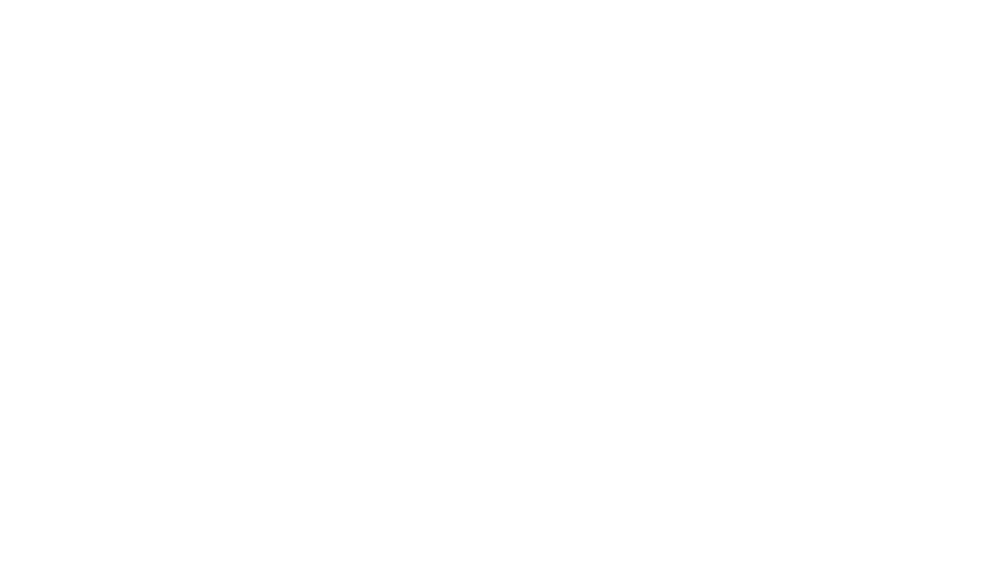
\includegraphics[height=3cm]{pics/dnet}
    
\includegraphics[height=3cm]{pics/logo_mendelu}
    
\includegraphics[height=3cm]{pics/logo_czechglobe}
    %\href{mailto:mikhailov.s@czechglobe.cz}{mikhailov.s@czechglobe.cz}
    % (can be left out to remove footer)
}

% use this to include logos on the left and/or right side of the header:
%\logoleft{
\includegraphics[height=7cm]{pics/logo_mendelu}}
%\logoright{
\includegraphics[height=5cm]{pics/logo_czechglobe}}

\begin{document}

\begin{frame}[t]
\begin{columns}[t]

%\separatorcolumn

\begin{column}{\colwidth}

\begin{alertblock}{Hypotheses and questions}
    We studied \textit{Pinus sylvestris} L. (Scots pine) xylem formation dynamics for two consecutive years, 2020 and 2021, on two research plots (150--350 m asl), representing managed Scots pine stands of different ages in the south of the Czech Republic -- 40 years of age (\textbf{young}) and 100 years of age (\textbf{old}).
    \begin{enumerate}
        \item What are the variation ranges of Scots pine cell morphology parameters under the drought stress?
        \item What is the threshold value for the number of cells, radial dimension of tracheids, and tree ring width to which these variables can decline without tree dieback?
        \item To what extent can Scots pine trees withstand water deficit stress, and does observation at the cellular level improve this determination?
        \item Is the same mechanism revealed as a reaction to drought stress regardless of tree age?
    \end{enumerate}
\end{alertblock}

\begin{block}{Methodology}
    \heading{Dendroclimatology}
        Retrospective growth analysis over the entire tree lifespan (12 trees); tree ring width (TRW) measurements, cross-dating, standardization by fitting the Hugershoff function, chronology building (Figure \ref{fig:hf}); climate--growth relationships: response and correlation function with T\textsubscript{avg}, P\textsubscript{sum}, SPEI\textsubscript{1}.
    \heading{Xylogenesis}
        Following the xylem formation dynamics (6 trees); weekly microcore sampling, sample preparation, number of cells in each differentiation phase were measured under the light microscope with 10--20x magnification, the phases: i) enlarging; ii) cell-wall thickening; iii) maturation.
    \heading{Xylem morphology}
        Quantitative wood anatomy (6 trees); captured images of the last two fully-formed annual rings (2020 and 2021), image batch processing with ImageMagick, measurements with ImageJ: continuous sequence of lumen diameter and cell wall thickness (CWT) (Figure \ref{fig:xmg}).
    \heading{Climatic data}
        Daily (site): T, RH, \Psi\textsubscript{Soil}, sap flow (Figure \ref{fig:sap}). Monthly (external): T\textsubscript{avg}, P\textsubscript{sum}, SPEI\textsubscript{1}.
        \begin{figure}
            \centering 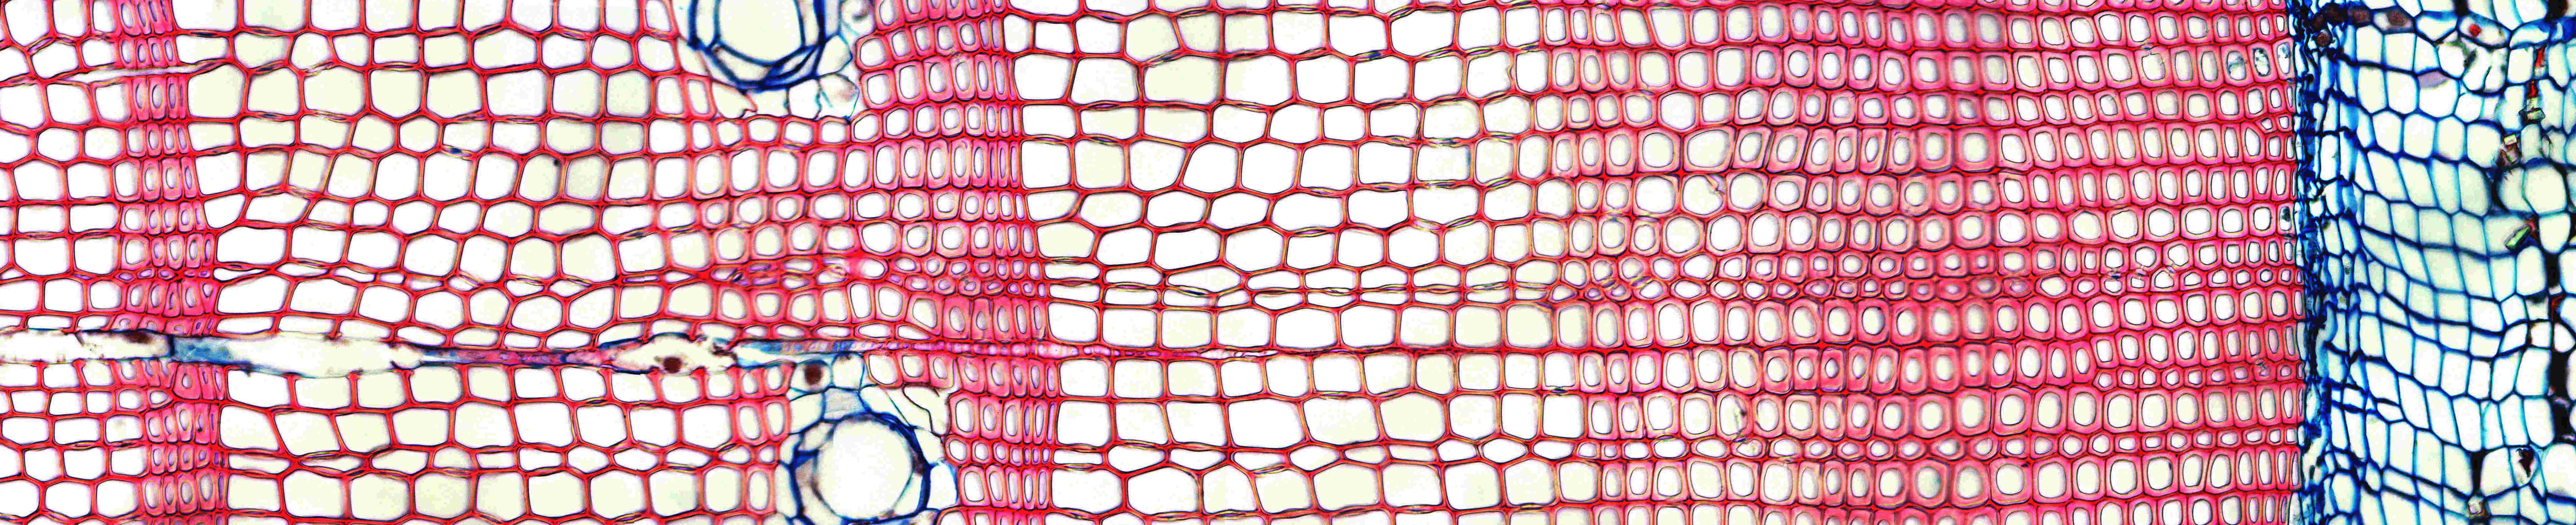
\includegraphics[width=1\textwidth]{pics/sob}
            \caption{Two consecutive annual rings from 2020 and 2021 (old stand), 20x magnification. Cambium and phloem are on the right in blue}
            \label{fig:sob}
        \end{figure}
\end{block}

\begin{block}{Drought stress}
        \begin{figure}
            \centering \includegraphics[width=1\textwidth]{pics/sap}
            \caption{Sap flow during 2020 and 2021. The old stand appeared to be more sensitive to dropping water availability in soil}
            \label{fig:sap}
        \end{figure}
\end{block}

\begin{block}{What is next?}
    \raggedleft
    \begin{enumerate}
        \item To establish functional dependency between xylem formation and environmental factors.
        \item To explain the effect of age on xylem formation under drought.
    \end{enumerate}
\end{block}

\end{column}

%\separatorcolumn

\begin{column}{\colwidth}

\begin{block}{Results}
    \heading{Tree ring width}
        \begin{figure}
            \centering \includegraphics[width=1\textwidth]{pics/hf}
            \caption{Inter-annual growth variability. Raw (left, Huggershoff function curve fitting the age trend) and indexed (right) TRW chronologies, where TRW -- tree ring width, \si{mm}; RWI -- ring width index (low frequency age trend is removed)}
            \label{fig:hf}
        \end{figure}
    \heading{Xylo- \& morphogenesis}
        \begin{figure}
            \centering 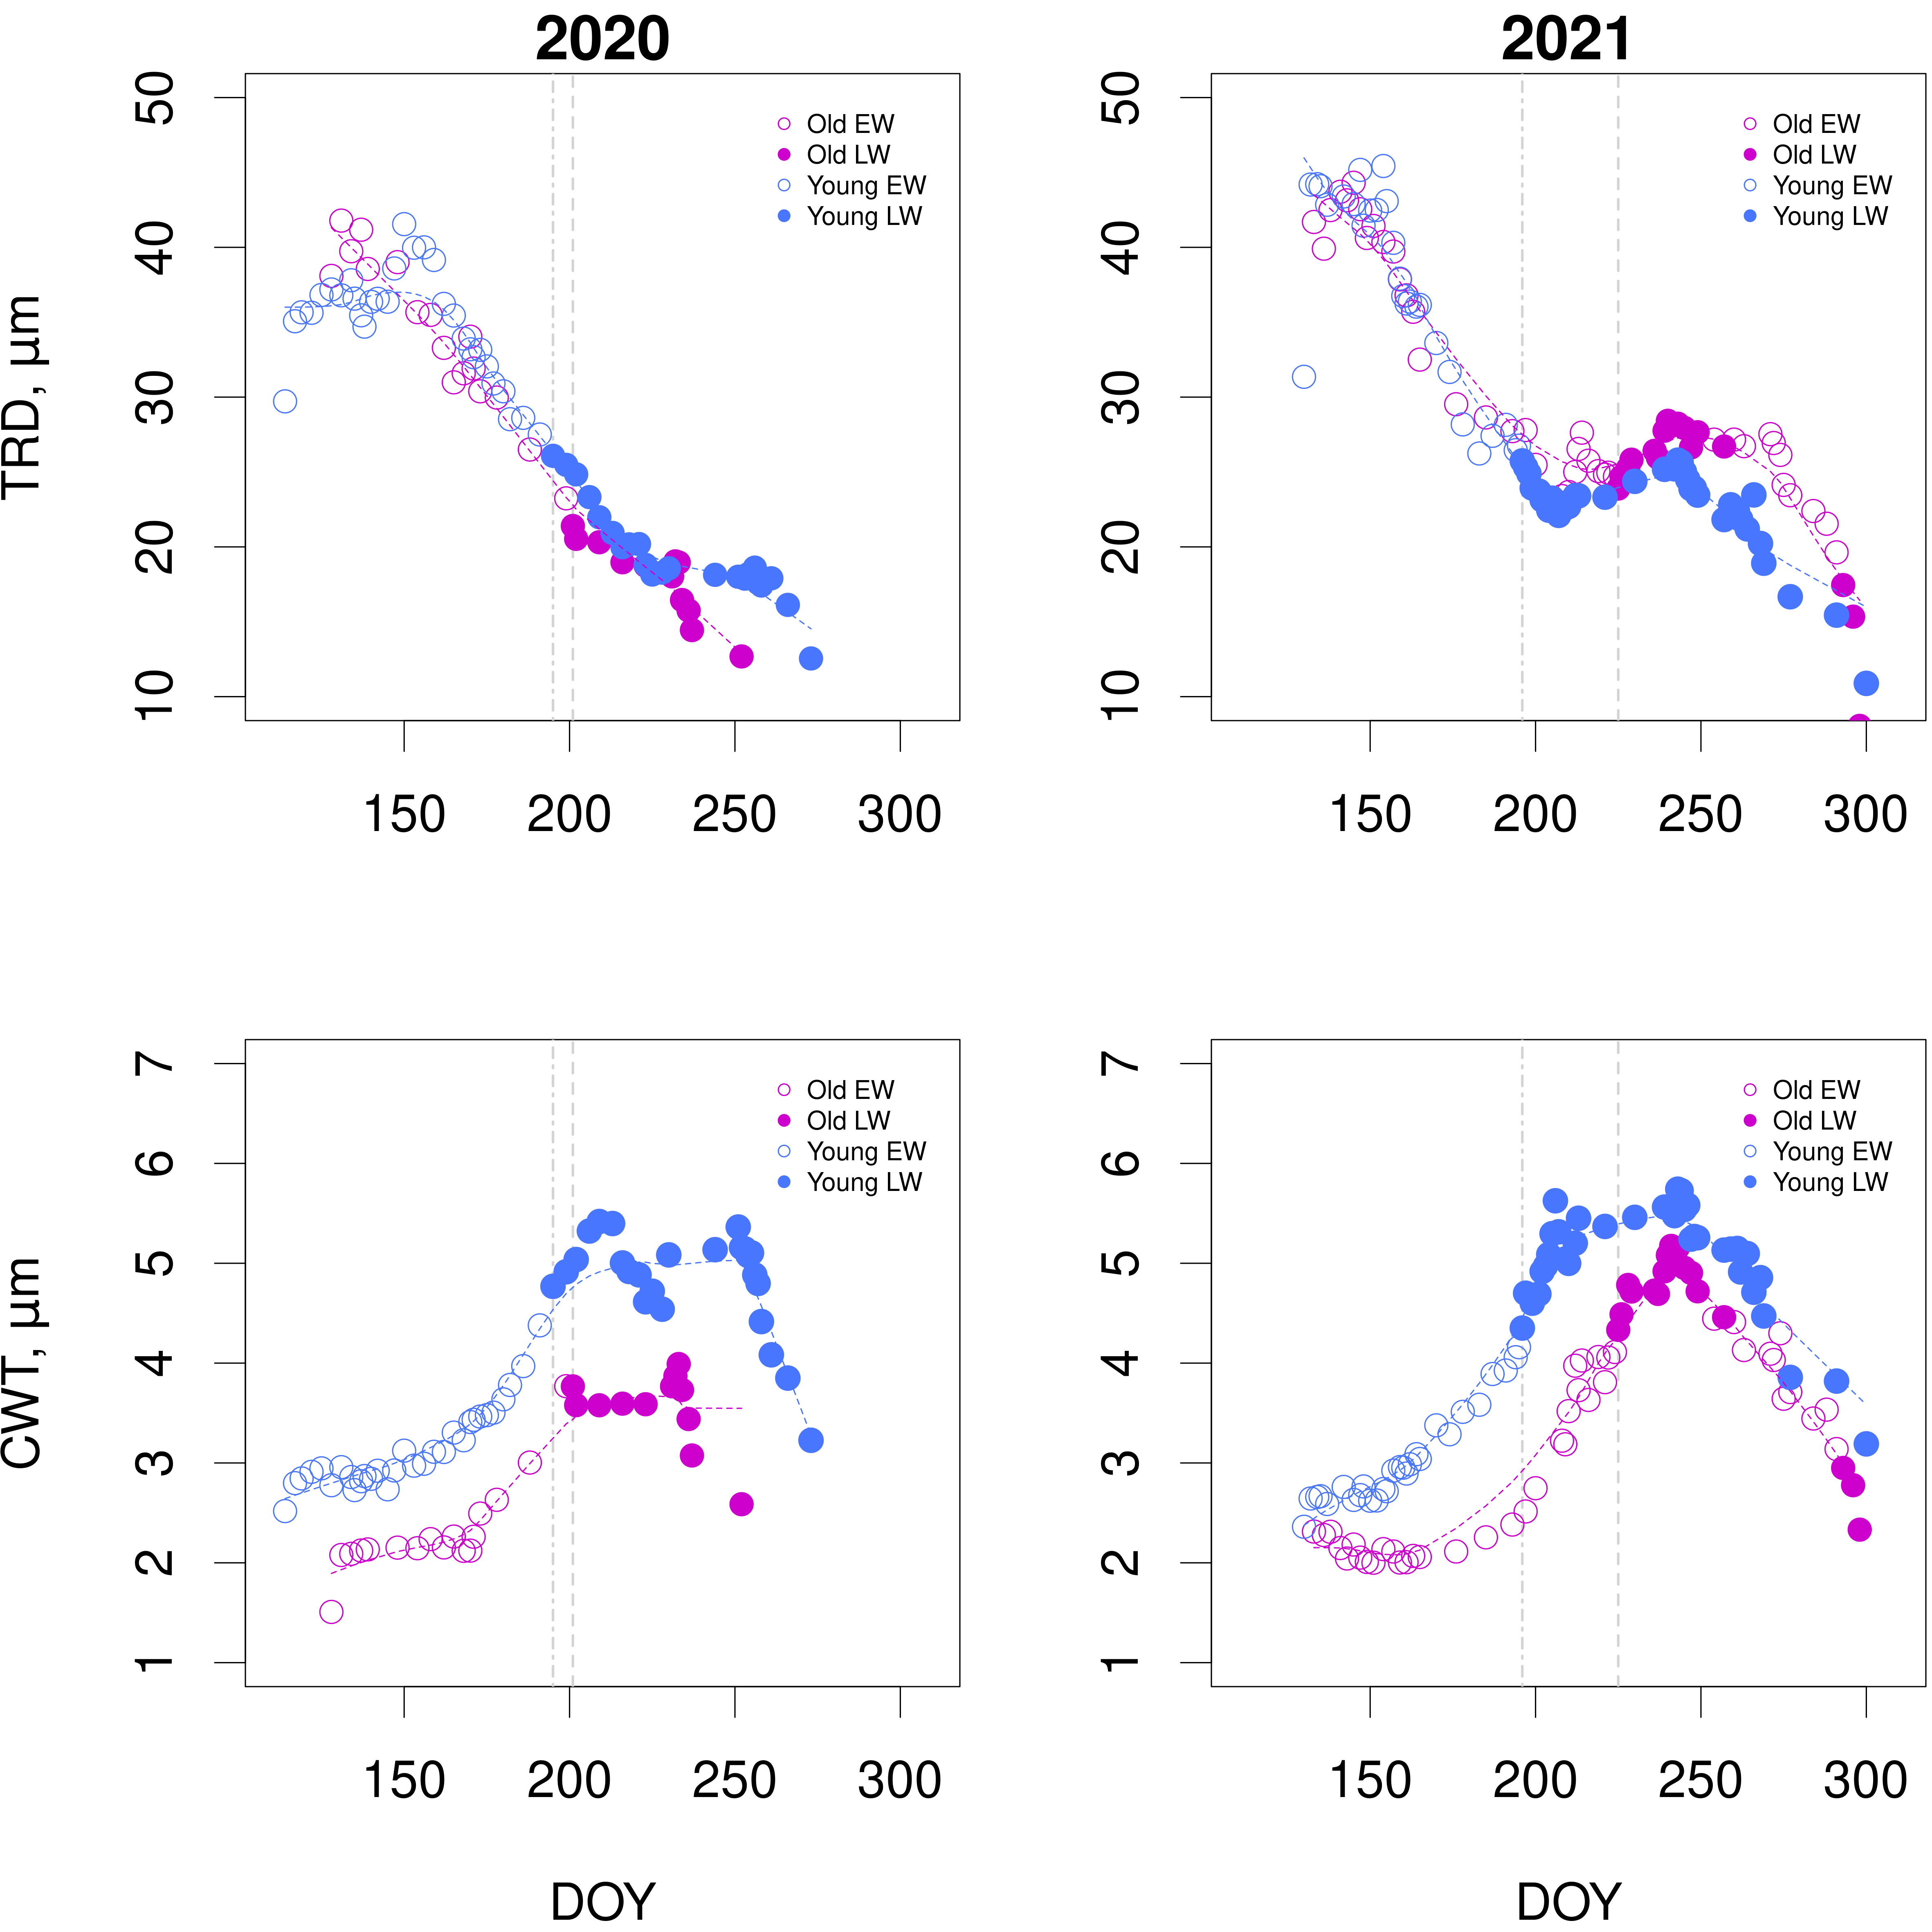
\includegraphics[width=1\textwidth]{pics/xmg}
            \caption{Intra-annual growth variability. Morphology metrics dated over xylogenesis, where TRD -- tracheid radial diameter, \si{\micro\meter}; CWT -- cell wall thickness, \si{\micro\meter}; DOY -- day of the year when the process of cell wall thickening began (i.e., TRD has already been fixed); EW -- early wood; LW -- late wood (classified according to Mork's criteria); vertical lines are borders between EW/LW border}
            \label{fig:xmg}
        \end{figure}
\end{block}

\begin{block}{Conclusions}
    \begin{enumerate}
        \item Number of cells and TRW differed both in young and old stand and under different levels of soil water availability.
        \item In both stands growth processes occurred within the following thresholds: TRD 10---45 \si{\micro\meter}; CWT 2---6 \si{\micro\meter}; TRW \sim1 \si{mm}. The old stand revealed maximum CWT decline up to 4 \si{\micro\meter} in 2020 and expressed cell wall thickening time delay in both years.
        \item TRW did not reveal drastic growth decline associated with drought. Though, on cellular level of observation the old stand appeared to be more responsive due to CWT adjustment.
        \item It is still unclear whether young and old stand share the same mechanism as a reaction to drought stress.
    \end{enumerate}
\end{block}

\end{column}
\end{columns}

%\begin{columns}[c]
%\begin{column}{0.96\paperwidth}
%
%\end{column}
%
%%\separatorcolumn
%
%\end{columns}
\end{frame}

\end{document}
